% Setup - do not change
\documentclass[11pt]{article}
\usepackage[top=0.9in, left=0.9in, bottom=0.9in, right=0.9in]{geometry} 
\usepackage{parskip}

\usepackage[english]{babel}
\usepackage[utf8]{inputenc}
\usepackage{amsmath,amsthm,amssymb,graphicx,pdfpages,lipsum,hyperref}
\usepackage[none]{hyphenat}
\usepackage{csquotes}

\graphicspath{ {./plots/} }

\setlength\parindent{0pt}
%%%%%%%%%%%%%%%%%%%%%%%%%%%%%%%%%%%%%%%%%%%%%%%%%%%%%%%%%%%%%%%%%%%
% add other packages here if required

%% Bibliography are specified in this file. You can also choose inline bib style if you want to. But make sure your citation style is consistent (and proper)
% For more details on citation: https://library.unimelb.edu.au/recite
\usepackage[sorting = none]{biblatex}
\addbibresource{references.bib}

%%%%%%%%%%%%%%%%%%%%%%%%%%%%%%%%%%%%%%%%%%%%%%%%%%%%%%%%%%%%%%%%%%% the '%' symbol denotes comments

% Begin document creation
% DELETE THE \lipsum PLACEHOLDERS WHEN YOU BEGIN
\title{\textbf{Insert} \\ Insert Subtitle}
\author{
Toomas Roosma \\
Student ID: 1381691 \\
%% Replace the link with your github repo
% 1. Remember to escape underscore in the link.
% 2. Remember to include the commit you want to submit in the link
\href{https://github.com/MAST30034-Applied-Data-Science/mast30034-project-1-ToomasRo/commit/68eb95dd343f163fd64bdcbf79bc71494db85056}{Github repo with commit}
}

\begin{document}
\maketitle

\section{Introduction}
% Link to a 30 min tutorial if you require revision: https://www.overleaf.com/learn/latex/Learn_LaTeX_in_30_minutes
In  New York City, the yellow taxicabs are a widely recognised symbols of the city. 
With the arrival of ridesharing services as Uber and Lyft in 2011 \cite{uberStartDate} and 2014 \cite{lyftStartDate} , the Taxi and Limousine Commission (TLC) has been forced to adapt to the new 
gig economy. With the introduction of e-hailing apps and green taxis, TLC has already made steps to adapt. This report
assumes the perspective of a taxi or rideshare company with the objective of forecasting demand for pickups in various locations around NYC.
Linear regression will be used to predict demand, based on data provided by the TLC from 2017 to 2019. This project aims to be also beneficial for taxi drivers, giving them insights, when to work and when not, giving better control over their work time. Yellow and green taxi data has been used, and they will be collectively referred to as taxi services.


\iffalse
TODO vist siia tuleb kirjutada kõike eeldused:
    - ainult sõidu alustamisel olnud ilm on oluline
    - kogu nyc ilm on sama
    - öelda miks ei kasuta 2020+, sest koroona ja muudab, eeldan et maailm muutub tagasi normi

    - introduction 1 mark point: I used 2018data to predict x using x. 
\fi

% use \textbf{} for bold text and \textit{} for italic. 


% You can have \section{}, \subsection{}, and \subsubsection{}
\section{Preprocessing, Analysis, and Geospatial Visualisation}

\subsection{Datasets}
This report uses mainly the taxi trip data provided by the New York City Taxi and Limousine Commission (NYCTLC) \cite{nyctlcData}. Files detailing the outlines of different taxi zones were also provided by the NYCTLC and used for visualisation purposes.

Weather data from LaGuardia Airport recorded by the United States National Center for Environmental Information's (NCEI) Integrated Global Surface dataset \cite{weatherData} was combined with the previously mentioned dataset. This work makes the assumption, that the weather at the moment when the decision to hail a taxi is done, has significant importance, whether or not the consumer will hail a taxi or not. It is also assumed, that the weather at the time of dropoff does not matter, because taxis are mainly used to circulate from door to door.

\subsection{Preprocessing}

\subsubsection{Dataset range selection}

We are working on the assumption that people are more pepared for bad weather during winter months, so only data from summer months (june, july and august) was used. Since 2017, the ride sharing companies Uber and Lyft have been required to share and publish drop-off date/time and locations \cite{tripUserGuide}. Both these companies have undeniably have aquired significant importance in the ride service providing scene in NYC, so data from 2017 and onwards was used. 
% (XXXtodo visualise green, yellow, fhv usage in NYC).

On the other end, data from 2020 and onwards was not used due to the lockdown and subsequent restriction put in place by NYC authorities. This means, that summer 2019 the last year included in this study. The world has since slowly gone back to normal, but as seen on the overall model performance in 2021, this return has not been completed. To see how the model performed one year after the global pandemic started, see section \ref{discussion}. After all the preprocessing, we were left with $271934805$ unique taxi trip entries.



\subsubsection{Feature selection}

Although the all the yearly datasets provided by the NYCTLC are said to follow one standard, they are not consistent with each other. There are also some outliers who do not follow the given structure. 

The weather data recorded at the LaGuardia airport by the NCEI \cite{weatherDataGuide} contains many irrelevant fields for this analysis, like monthly averages and quality control codes. There are also datafields that are too local or not applicable for taxi services at the selected period, like wave height and snow accumulations. The type of daily present weather being reported was discarded due to conveying to little differential information about each hour. Cloud coverage was repurposed from a ordinal variable to discrete, as cloud coverage of missing hours was imputed from neighboring hours. Other weather attributes like windspeed and temperature were imputed in a similar fashion.

\subsubsection{Eliminating outliers}

% (XXTODO siia võiks leida ilusasti numbrid)

\textbf{Trips with invalid pickup and drop-off location ID} were discarded from the dataset, as the shapefiles defined only location IDs in the range 1-263.

\textbf{Trips with pickup date outside the defined range} were discarded. Drop-offs outside the selected range were left in, because we are interested in predicting pickups.

\textbf{Trips with negative duration} were detected and discarded.

\textbf{Trips with distances over 6 hours} were discarded from the dataset. According to google maps, a trip between Totenville and Wakefield (extremities of area of study) would take only 2h during rush hours.

\textbf{Trips with distances over 150 miles} were discarded from the dataset, as the the average trip length was 3 miles with a standard deviation of 7 miles. The same trip mentioned previously is 46 miles one way.

\textbf{Trips with no passenger} data or zero passengers were removed.


The following data was retained from the taxi dataset:
\begin{itemize}
    \item Month, day and hour
    \item Weekday
    \item Pickup location ID
\end{itemize}

And the following from the weather dataset:
\begin{itemize}
    \item Wind speed
    \item Visibility
    \item Air temperature
    \item Dew point
    \item Atmospheric pressure
    \item Cloud coverage
\end{itemize}



%[XXTODO] - vähemalt 1 good geospacial Visualisation

\iffalse
Example code for figures:
% the [h] ensures your figure is inline at the location and not displayed on some other page
\begin{figure}[h]
    % change the scale multiplier to make the figures smaller or larger
    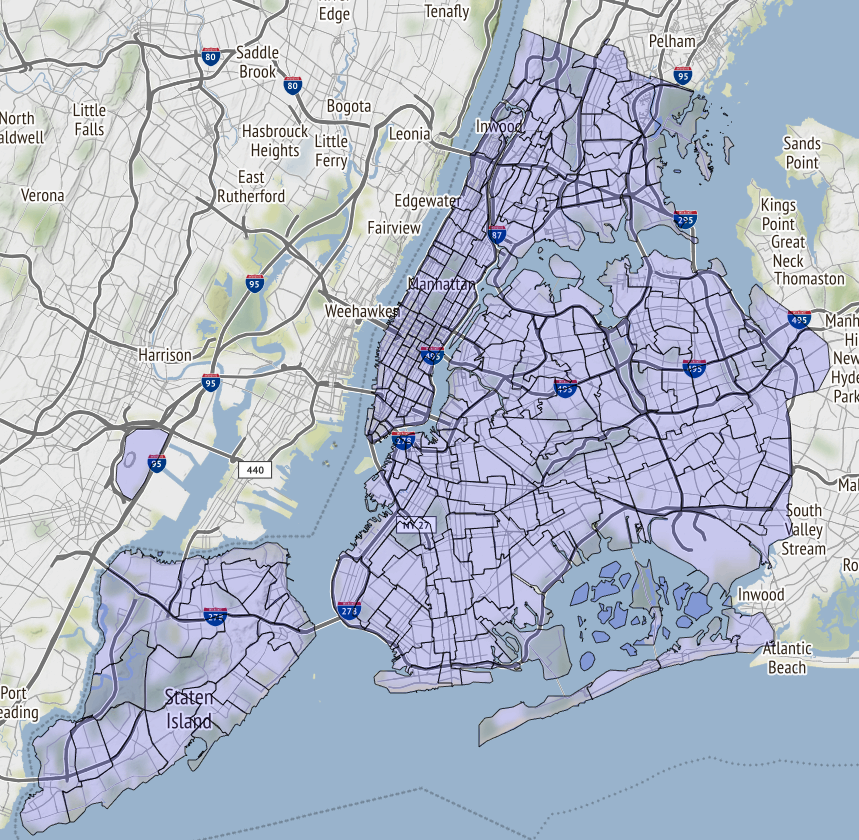
\includegraphics[width=0.35\textwidth]{nyc_map.PNG}
    % this ensures your figures are centered where possible
    \centering
    \caption{Some caption} % refer to this image as (Figure 1)
\end{figure}
\fi

\section{Modelling}

\iffalse
    TODO:
    - võib olla ka random forrest, ei pea olema mathematical (linear vms)
    - esimene hinne: tuleb justify miks võtad. (nt linear model falsefully classifieb, ja seejärel teed penalised ja läheb halvemaks, siis teist ei kasuta)
        - tuleb 2 strictly erinevat, kui üks lin mod c teine, siis ei loe

    - tuleb reference provideda??? okei kui see pole prereq jooksul kaetud, ft küsida
    - conclusion: nt airport areas are special

- categorical data peab olema onehot encoded (weather, locationIDs)
\fi


\section{Recommendations}


\subsection{Discussion} \label{discussion}

The linear regression model performs surprisingly well, as the pickup number per hour per zone varies greatly (mean of 764 and standard deviation of 1024). The most apropriate metric to grade our model is Mean Absolute Error (MAE), because of how easy it is to interprete. Our model achieved a MAE of 123, with an $R^2$ of 0.49. This means, that on average the model predicts the demand better than humans.

\begin{figure}[h]
    % change the scale multiplier to make the figures smaller or larger
    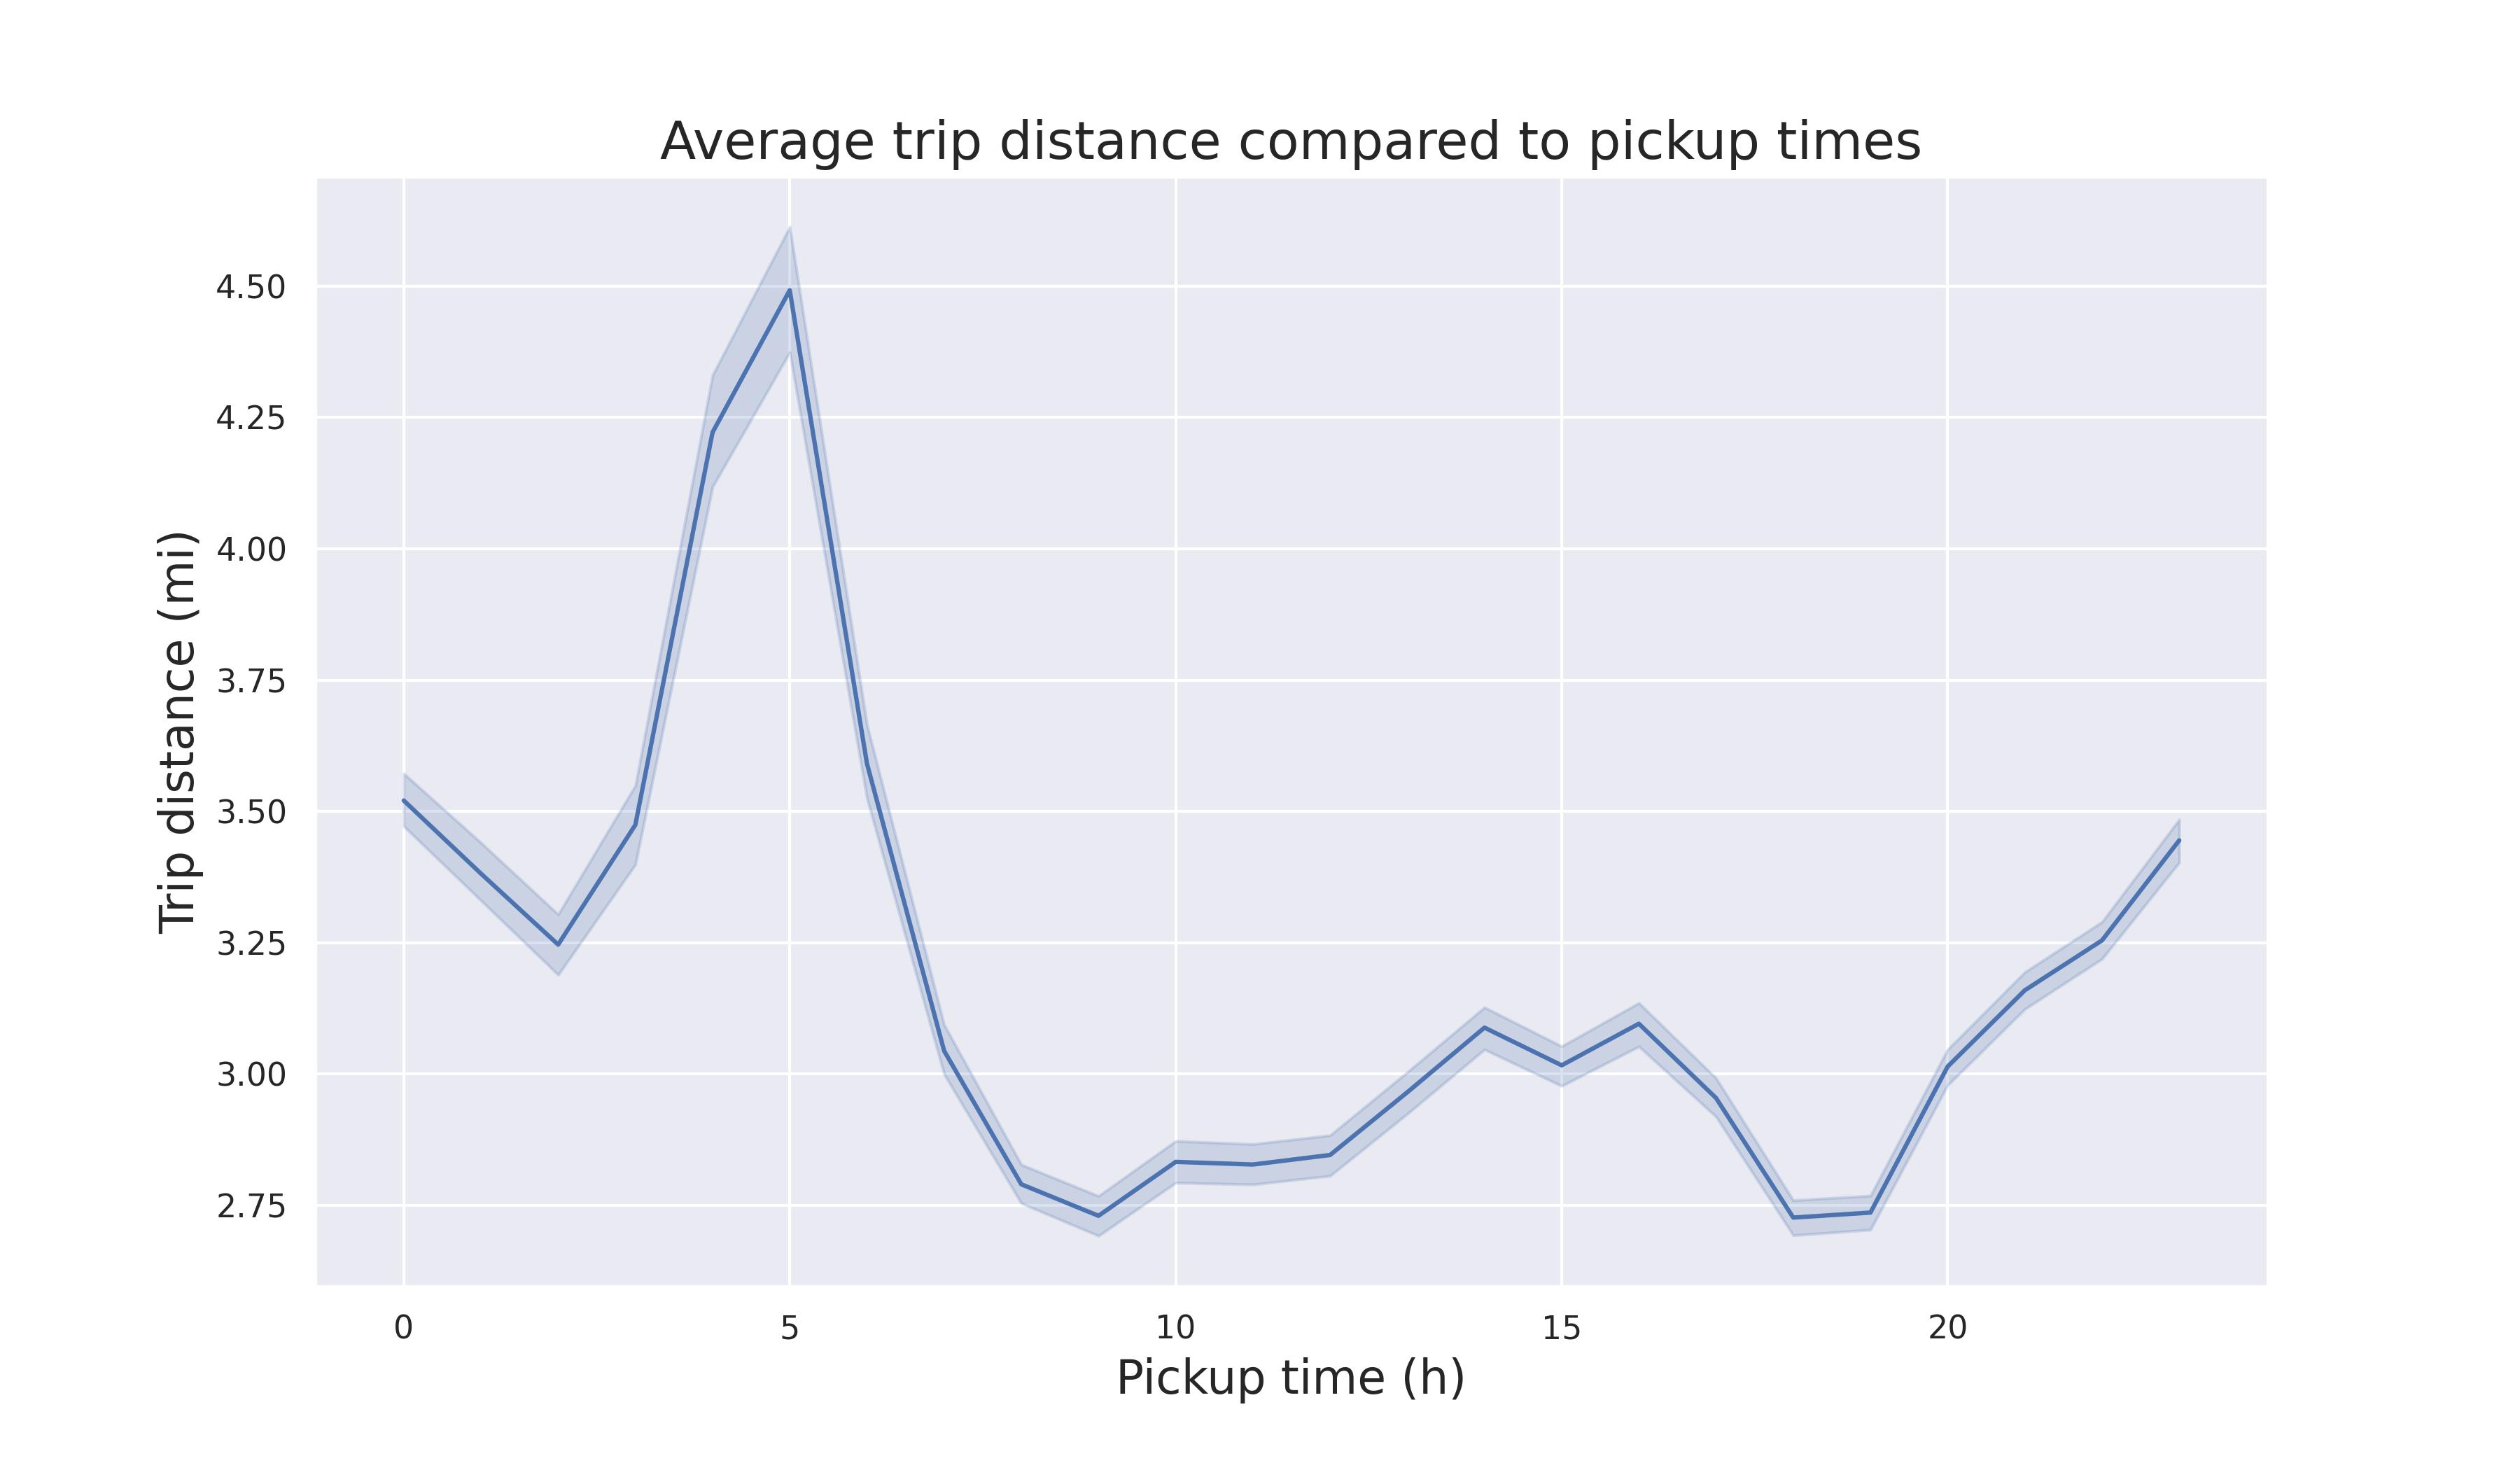
\includegraphics[width=0.65\textwidth]{pickuptime_distance.jpeg}
    % this ensures your figures are centered where possible
    \centering
    \caption{Some caption} % refer to this image as (Figure 1)
\end{figure}

\iffalse
TODO: 
    -ei ole summary of entire paper
\fi


\section{Conclusion}

This model proved itself interesting enough to pursue futher research. However, due to the lack of sharing information from other ride sharing companies like Uber, predicting the demand is limited to weather data. With data from them, more precise amounts of passengers could be estimated, which can also be used as a proxy for demand.


\clearpage

% BEGIN REFERENCES SECTION
\printbibliography

\end{document}

\iffalse

Notes from tutorial: 

Alguses on vaja kõik abreviationid lahti kirjutada ehk (e) sulgudesse panna e edasi võib niisama kasutada
higher level overview sentence(paragraf)
deep neural networki oleks vaja citation lisada kust see tuleb
further defining assumptions and abbr

mainida lausekesega dataset, vb preproc all

range justification on suhteliselt common knowledge, 3-4 rida probs teeb asja ära. kui ruumi jääb üle siis saab pikemaks teha + grafics
dataset size võiks mainida + amount of features

preproc: alustada tldr (iga paragraafi)
DO NOT MAKE CLAIMS THAT HAVE NO SUPPORT

feature selection: do not make a list with every attribute and then the reasoning keeping/discarding
THROW AWAY YEAR, SO THAT it wokrs on future data as well


make sure that variable names on plots are readable (not n_pickups)
good size


regression model is not for classification

Lucase error analysis on hea, sest mudel kasutab nii aeg kui loc, siis ta fikseeris loc ja time ning analüüsis seda
\fi

\iffalse
reference läheb enne punkti ja tühikut pole enne punkti
\fi

\iffalse
Endale:
    - öelda et suvel on lastel puhkusem, seega taksojuhid äkki tahaksid päeva nendega veeta
    - kui saad keskmise vea suht madala, aga mõnel on kõrgem, siis limiti visualiseerimisel -75,+75 ja kirjelda seda suurte vigadega kohta (lucase fig6)
    - rääkida et FHV saab parema dataga opereerida, lihtsamini motiveerida sõitjaid peak houril (nt anda suurem cut vms) jne
    https://www.businessinsider.com/worst-time-to-hail-a-cab-in-nyc-2015-11
    - 
    - saab kasutada rigdge, OIS regression, GLM, 
    - report should not mention code at all (varibale names!)
    - mis on stepwise selection
\fi


\iffalse
halvad repordid:
    - plot really small, plot does not help (just say I removed outliers)
    - plot variables not renamed to human variables
    - dont put title: x-axis vs y-axis
    - scale: ära topi 0 ebanormaalsesse kohta (eg alguses või keskel)
    - discussion is not founded, just pasted results
    - ära tee pearson cor mat kui data pole continous

\fi